\documentclass[article,nojss]{jss}
\usepackage{amsmath,amssymb,booktabs}
\usepackage{graphicx}

%% The author's style rules forbid bold and italics in running text.
%% jss.cls sets package names in bold; they are set in roman here.
\renewcommand{\pkg}[1]{#1}

\newcommand{\tr}{\operatorname{tr}}
\newcommand{\vecop}{\operatorname{vec}}
\newcommand{\diag}{\operatorname{diag}}
\newcommand{\dimC}{\operatorname{dim}}

%% TODO: full postal address of the author.
\author{Nicolas Salas\\INRAE}
\title{\pkg{remlax}: Restricted Maximum Likelihood for Structured and
  Multi-Trait Linear Mixed Models on the Marginal Covariance or the Mixed
  Model Equations, on CPU and GPU}
\Plainauthor{Nicolas Salas}
\Plaintitle{remlax: REML for Structured and Multi-Trait Linear Mixed Models
  on CPU and GPU}
\Shorttitle{\pkg{remlax}: REML on CPU and GPU}

\Abstract{
Restricted maximum likelihood (REML) is the standard method to estimate
variance components in plant and animal breeding. The models in use combine
multi-trait covariances, known relationship matrices, spatial correlations and
weighted neighbour incidences. Software that covers this catalogue is
either commercial or restricted in structure. \pkg{remlax} is an \proglang{R}
package with a \proglang{Python} engine built on \pkg{JAX}. It evaluates the
same REML criterion on the marginal covariance $V$, differentiated by a
closed-form adjoint and automatic differentiation, or on Henderson's mixed
model equations, factorised by a supernodal sparse Cholesky decomposition with
selected inversion. Both forms run on CPU, and the dense computations also run
on GPU. The variance parameters are estimated by L-BFGS-B or by average
information REML with steps on the variance scale. Average information steps
keep unstructured covariance blocks on the positive semidefinite cone and
rotate them on its faces when the optimum is rank deficient. Every fit reports the
Newton decrement, the projected relative gradient and the spectrum of the
Hessian. Against \pkg{asreml}, \pkg{lme4}, \pkg{nlme}, \pkg{sommer} and
\pkg{pbkrtest}, 341 of 353 checks passed, and the 12 others were traced to
\pkg{asreml} stopping short of the optimum. On simulated genomic models, an
NVIDIA A100 fitted multi-trait unstructured and factor analytic models up to
49 times faster than \pkg{ASReml-R} on 8 CPU cores.
}
\Keywords{REML, average information, mixed model equations, selected
  inversion, GPU, \proglang{JAX}, multi-trait models, indirect genetic
  effects, \proglang{R}, \proglang{Python}}
\Plainkeywords{REML, average information, mixed model equations, selected
  inversion, GPU, JAX, multi-trait models, indirect genetic effects, R,
  Python}
\Address{
  Nicolas Salas\\
  INRAE\\
  E-mail: \email{nicolas.salas@supagro.fr}
}

\begin{document}
\maketitle

%% =========================================================================
\section{Introduction}\label{sec:intro}

Linear mixed models fitted by restricted maximum likelihood (REML) are the
standard tool for the estimation of variance components and the prediction of
breeding values \citep{patterson1971,henderson1975}. Breeding analyses rarely
use a single random factor. They combine unstructured or factor analytic
covariances between traits or environments \citep{smith2001}, genomic or
pedigree relationship matrices \citep{vanraden2008}, and separable
autoregressive fields for the spatial trend of a trial \citep{gilmour1997}.

Neighbour models add one more layer. The phenotype of a plant or an animal
then depends on the genotypes of its neighbours through indirect genetic
effects \citep{muir2005,bijma2007}. Their incidence is a
weighted matrix, and the covariance between direct and indirect effects is
unstructured. In mixtures of species, one such term is needed per species and
per type of neighbour, so that a single model can carry tens of terms and
hundreds of variance parameters \citep{salas2026}.

Average information REML on sparse mixed model equations is the reference
algorithm for these models \citep{gilmour1995,johnson1995}. \pkg{ASReml-R}
implements it with the widest catalogue of covariance structures
\citep{butler2023}, under a commercial licence. Among free packages,
\pkg{lme4} fits unstructured covariances per grouping factor, and has no
argument for a known relationship matrix \citep{lme4}. \pkg{sommer} accepts relationship matrices
and several traits and works on the marginal covariance
\citep{sommer}. \pkg{kmmr} recently combined supernodal sparse factorisation
on CPU with a dense Schur complement on GPU \citep{melsen2026}. A free solver
that covers the structures of \pkg{ASReml-R}, weighted incidences and
multi-trait terms, on CPU and on GPU, has remained missing.

Here, we present \pkg{remlax}, an \proglang{R} package whose computations run
in a \proglang{Python} engine built on \pkg{JAX} \citep{jax2018}. The same
model is fitted either on the marginal covariance $V$ or on the mixed model
equations, with the same parameters and the same likelihood. In the dense
form, a closed-form adjoint differentiates $V$, and the computation runs
unchanged on CPU or GPU. The mixed model form uses a supernodal sparse Cholesky factorisation, a
selected inversion and, on GPU, a dense inversion. Average information steps
are taken on the variance scale, and a rank-deficient unstructured block is
handled on the faces of the positive semidefinite cone. Every fit reports a
set of convergence diagnostics.

Section~\ref{sec:model} states the model and its parametrisation, and
Section~\ref{sec:reml} gives the restricted likelihood in both forms, its
gradient and the average information step. The engines, the optimisers and
the inference follow in Section~\ref{sec:computation}.
Section~\ref{sec:software} presents the \proglang{R} interface with an
example. The validation and the benchmarks are reported in
Sections~\ref{sec:validation} and~\ref{sec:benchmarks}, and
Section~\ref{sec:limits} closes with limitations and availability.

%% =========================================================================
\section{Model and notation}\label{sec:model}

\subsection{The linear mixed model}

\pkg{remlax} fits the linear mixed model
\begin{equation}\label{eq:lmm}
  y = X\beta + \sum_{k=1}^{c} Z_k u_k + e,
  \qquad
  u_k \sim \mathcal{N}(0, G_k), \quad G_k = \Sigma_k \otimes K_k,
  \qquad
  e \sim \mathcal{N}(0, R),
\end{equation}
where $y$ holds $n$ observations, $X$ is an $n \times f$ design matrix of full
column rank and $\beta$ the fixed effects. A random term $k$ groups $t_k$
incidence matrices $Z_{k1}, \dots, Z_{kt_k}$ of size $n \times q_k$ that share
the same $q_k$ levels, and $Z_k = [Z_{k1} \cdots Z_{kt_k}]$. The $t_k \times
t_k$ matrix $\Sigma_k$ is a covariance between the columns of the term. Its
levels are linked by the $q_k \times q_k$ matrix $K_k$, either known, such as a
genomic relationship matrix, or a correlation matrix $C_k(\rho_k)$ with its
own parameters. The level index varies fastest in $u_k$ and in the columns of
$Z_k$, as in the Kronecker product. Terms are independent,
so that $G = \bigoplus_k G_k$.

This form covers the usual models. A random factor has $t_k = 1$, $\Sigma_k =
\sigma_k^2$ and $K_k = I$. For a genomic BLUP, $K_k$ is a relationship
matrix. A multi-trait or multi-environment term has one column per trait, each
$Z_{kj}$ being the genotype incidence restricted to trait $j$. In a direct and
indirect genetic effects term, $t_k = 2$, with $Z_{k1}$ the incidence of the
own genotype and $Z_{k2}$ a weighted incidence of the neighbours. Spatial
fields take $K_k$ as a separable AR(1) correlation over rows and columns.

The residual is a direct sum over $S$ sections that partition the
observations. Within section $s$, the covariance between observations $i$ and
$j$ is
\begin{equation}\label{eq:resid}
  R_{ij} = \Sigma^{e}_{s}[\tau(i), \tau(j)]\; C_s[\upsilon(i), \upsilon(j)],
\end{equation}
where $\tau(i)$ is the trait and $\upsilon(i)$ the unit of observation $i$.
In matrix form, $R_s = T_s (\Sigma^{e}_s \otimes C_s) T_s^\top$, with $T_s$ the
selection of the observed (trait, unit) cells. An independent residual has
$\Sigma^e_s = \sigma^2_s$ and $C_s = I$. A multi-trait residual has an
unstructured $\Sigma^e_s$ with $C_s = I$, and a separable field has $C_s =
C_{\rm row} \otimes C_{\rm col}$. The marginal covariance of $y$ is
\begin{equation}\label{eq:V}
  V = \sum_{k=1}^{c} Z_k (\Sigma_k \otimes K_k) Z_k^\top + R .
\end{equation}

\subsection{Covariance structures}

Table~\ref{tab:sigma} lists the structures available for $\Sigma_k$. They
follow the catalogue of \pkg{ASReml-R} \citep{butler2023}. The structure
between levels contributes a correlation matrix only, and the variance lives
in $\Sigma_k$. It follows the decomposition $\Sigma = D C D$ of the
\pkg{ASReml-R} manual, so that an \code{ar1v} of \pkg{ASReml-R} is written
\code{ar1(f)} and an \code{ar1h} is \code{ar1(f, struct = "diag")}.

\begin{table}[t]
\centering
\small
\begin{tabular}{lllc}
\toprule
\pkg{remlax} & \pkg{ASReml-R} & $\Sigma$ & Parameters \\
\midrule
\code{iid}     & \code{idv}     & $\sigma^2 I_t$ & $1$ \\
\code{diag}    & \code{idh}     & $\diag(\sigma^2_j)$ & $t$ \\
\code{us}      & \code{corgh}   & $LL^\top$, $L$ lower triangular & $t(t+1)/2$ \\
\code{fa(m)}   & \code{fa(m)}   & $\Lambda\Lambda^\top + \diag(\psi^2)$ & $\ell(t,m) + t$ \\
\code{rr(m)}   & \code{rr(m)}   & $\Gamma\Gamma^\top$, rank $m$ & $\ell(t,m)$ \\
\code{chol(b)} & \code{chol(b)} & $LDL^\top$, $L$ unit lower triangular, band $b$ & $(b+1)(t-b/2)$ \\
\code{ante(b)} & \code{ante(b)} & $\Sigma^{-1} = UDU^\top$, $U$ unit upper triangular, band $b$ & $(b+1)(t-b/2)$ \\
\code{corh}    & \code{corh}    & $D C D$, $C$ uniform correlation & $t+1$ \\
\bottomrule
\end{tabular}
\caption{\label{tab:sigma}Covariance structures for $\Sigma$ over $t$
columns. $\ell(t,m) = \sum_{i=1}^{t} \min(i,m)$ counts the free entries of a
lower trapezoidal $t \times m$ matrix.}
\end{table}

The loading matrices $\Lambda$ and $\Gamma$ are lower trapezoidal. Without this
constraint they are defined up to an $m \times m$ rotation, and the
likelihood has a flat ridge of dimension $m(m-1)/2$. The count of \code{rr(m)}
is therefore smaller by $m(m-1)/2$ than the $tm$ of the \pkg{ASReml-R} manual,
with the same fitted model. A rank-deficient \code{rr} is admissible because
$V$ is assembled from factors (Section~\ref{sec:dense}), so that a singular
$\Sigma_k$ does not make $V$ singular when another term or the residual
completes it.

The structures between levels include the stationary families \code{ar1},
\code{ar2}, \code{ar3}, \code{sar}, \code{ma1}, \code{ma2}, \code{arma} and the
banded correlation \code{corb}. They also include a uniform correlation
\code{cor}, a general correlation \code{corg}, and metric kernels on one or two
coordinates. The metric kernels are the exponential and Gaussian families
(\code{exp}, \code{gau}, \code{iexp}, \code{igau}, \code{ieuc}, \code{aexp},
\code{agau}), the range kernels \code{lvr}, \code{sph} and \code{cir}, and the
anisotropic Mat\'ern correlation of \citet{haskard2007}. Separable products
such as \code{ar1(row):ar1(col)} and user-written kernels (\code{own}) complete
the catalogue. A user kernel is an expression in the distances and the
parameters, passed as a string and differentiated automatically.

\subsection{Parametrisation}\label{sec:param}

The variance parameters form one vector $\theta \in \mathbb{R}^p$. For each
term, the parameters of $\Sigma_k$ come first and those of the level
structure next. Terms follow in their order of declaration, then the
residual sections. The parametrisation is unconstrained, and positive
definiteness holds by construction. For an unstructured block,
\begin{equation}\label{eq:chol}
  \Sigma = LL^\top, \qquad L_{ii} = \exp(\theta_{ii}), \qquad L_{ij} =
  \theta_{ij} \quad (i > j),
\end{equation}
so that the diagonal of the Cholesky factor is carried on the log scale. A
variance is $\sigma^2 = \exp(2\theta)$, and a specific variance of a factor
analytic structure is $\psi^2 = \exp(2\theta)$. An autoregressive correlation
is $\rho = \tanh\theta$. A metric correlation raised to a distance is $\rho =
|\tanh\theta|$, so its sign is not identified and is reported positive. Ranges
and Mat\'ern shapes are $\exp\theta$. The uniform correlation of \code{cor} and
\code{corh} is a $\tanh$ rescaled onto $(-1/(q-1), 1)$, its exact interval of
positive definiteness. For \code{ar2} and \code{ar3}, the parameters are the
partial autocorrelations, each in $\tanh$, mapped to the autoregressive
coefficients by the Levinson--Durbin recursion. This bijection
covers exactly the stationarity region.

Every element of $\theta$ is bounded to $[-12, 12]$. Positivity does not need
these bounds. They stop a variance from escaping towards $\exp(-\infty)$,
where its gradient vanishes and the point cannot be told apart from an
optimum.

%% =========================================================================
\section{Restricted likelihood and its derivatives}\label{sec:reml}

\subsection{The marginal form}

The restricted log-likelihood $\ell_R$ satisfies
\begin{equation}\label{eq:remlV}
  -2\ell_R(\theta) = (n-f)\log 2\pi + \log|V| + \log|X^\top V^{-1} X| +
  y^\top P y,
\end{equation}
with
\begin{equation}\label{eq:P}
  P = V^{-1} - V^{-1}X(X^\top V^{-1}X)^{-1}X^\top V^{-1}.
\end{equation}
\pkg{remlax} keeps the constant $(n-f)\log 2\pi$, as \pkg{lme4} does.
\pkg{ASReml-R} omits it, and every fit also returns the log-likelihood in that
convention.

The criterion depends on $X$ through its column space only, up to a constant.
With the reduced QR decomposition $X = Q_X R_X$,
\begin{equation}\label{eq:qr}
  \log|X^\top V^{-1} X| = \log|Q_X^\top V^{-1} Q_X| + 2\log|\det R_X| .
\end{equation}
Both engines work with $Q_X$. A covariate on a large scale, such as a date,
then costs no precision in $\log|X^\top V^{-1}X|$.

The derivative of \eqref{eq:remlV} with respect to $V$ has the closed form
\begin{equation}\label{eq:adjoint}
  \bar V = \frac{\partial(-2\ell_R)}{\partial V} = P - (Py)(Py)^\top ,
\end{equation}
which gives the score of each parameter as
\begin{equation}\label{eq:scoreV}
  \frac{\partial(-2\ell_R)}{\partial\theta_i}
  = \tr(\bar V V_i) = \tr(P V_i) - y^\top P V_i P y,
  \qquad V_i = \frac{\partial V}{\partial\theta_i}.
\end{equation}
The dense engine supplies $\bar V$ as a custom reverse-mode rule, and automatic
differentiation propagates it through the code that builds $V$ from
$\theta$. Any smooth parametrisation of $V$ thus receives its gradient without
a hand-written derivative.

\subsection{The mixed model equations}

With $W = [X \; Z]$, $Z = [Z_1 \cdots Z_c]$ and $u$ the stacked random
effects, Henderson's mixed model equations \citep{henderson1975} are
\begin{equation}\label{eq:mme}
  C \begin{pmatrix}\hat\beta \\ \hat u\end{pmatrix} = W^\top R^{-1} y,
  \qquad
  C = W^\top R^{-1} W + \begin{pmatrix} 0 & 0 \\ 0 & G^{-1}\end{pmatrix}
    = \begin{pmatrix}
      X^\top R^{-1} X & X^\top R^{-1} Z \\
      Z^\top R^{-1} X & Z^\top R^{-1} Z + G^{-1}
    \end{pmatrix}.
\end{equation}
The order of $C$ is $m = f + \sum_k t_k q_k$, the number of fixed effects plus
the number of random levels over all columns. The criterion
\eqref{eq:remlV} takes the equivalent form
\begin{equation}\label{eq:remlC}
  -2\ell_R(\theta) = (n-f)\log 2\pi + \log|R| + \log|G| + \log|C| +
  y^\top P y,
\end{equation}
where
\begin{equation}\label{eq:yPy}
  y^\top P y = y^\top R^{-1}y - r^\top C^{-1} r,
  \qquad r = W^\top R^{-1} y,
\end{equation}
with $\log|G| = \sum_k \left(q_k \log|\Sigma_k| + t_k \log|K_k|\right)$ and
$G_k^{-1} = \Sigma_k^{-1} \otimes K_k^{-1}$. When $X$ is replaced by $Q_X$,
the term $2\log|\det R_X|$ of \eqref{eq:qr} is added. The marginal form costs
a factorisation of order $n$, and the mixed model form one of order $m$, which
is cheap when $C$ is sparse.

\subsection{Scores on the mixed model equations}

The mixed model engine first differentiates with respect to the entries of
each $\Sigma_k$ and the level parameters, where the formulas are simple. Let
$\hat U_k$ be the $q_k \times t_k$ matrix of BLUPs of term $k$, with
$\vecop(\hat U_k) = \hat u_k$. The block $C^{kk}$ of $C^{-1}$ that belongs to
term $k$ splits into $t_k^2$ blocks $C^{kk}_{ab}$ of size $q_k \times q_k$,
which define the $t_k \times t_k$ matrix of traces $(T_k)_{ab} =
\tr(K_k^{-1} C^{kk}_{ab})$ \citep{jensen1997,melsen2026}. With
\begin{equation}\label{eq:M}
  M_k = q_k \Sigma_k^{-1} - \Sigma_k^{-1}\left(T_k + \hat U_k^\top K_k^{-1}
  \hat U_k\right)\Sigma_k^{-1},
\end{equation}
the score of entry $\sigma_{ab}$ of $\Sigma_k$ is $(M_k)_{aa}$ when $a = b$
and $2(M_k)_{ab}$ otherwise. For a parameter $\rho$ of a parametrised level
correlation,
\begin{equation}\label{eq:scorerho}
  \frac{\partial(-2\ell_R)}{\partial\rho}
  = t_k \frac{\partial\log|K_k|}{\partial\rho}
  + \sum_{a,b} (\Sigma_k^{-1})_{ab}\,
    \tr\!\left(C^{kk}_{ab}\,\frac{\partial K_k^{-1}}{\partial\rho}\right)
  + \tr\!\left(\Sigma_k^{-1}\, \hat U_k^\top \frac{\partial
    K_k^{-1}}{\partial\rho} \hat U_k\right).
\end{equation}
For a residual section with parameter $\phi$ and residuals $\hat e = y -
W(\hat\beta^\top, \hat u^\top)^\top$,
\begin{equation}\label{eq:scoreR}
  \frac{\partial(-2\ell_R)}{\partial\phi}
  = \tr(R^{-1}R_\phi)
  - \tr\!\left(C^{-1} W^\top R^{-1} R_\phi R^{-1} W\right)
  - \hat e^\top R^{-1} R_\phi R^{-1} \hat e,
  \qquad R_\phi = \frac{\partial R}{\partial \phi}.
\end{equation}
A section without structure between units reduces \eqref{eq:scoreR} to small
matrices, one per pattern of observed traits. The traces in
\eqref{eq:M}--\eqref{eq:scoreR} need the entries of $C^{-1}$ on the pattern of
$C$ only. Scores $s$ in these internal coordinates are carried to $\theta$
by the Jacobian $J$ of the internal coordinates with respect to $\theta$,
$g_\theta = J^\top s$, which \pkg{JAX} computes exactly.

\subsection{The average information matrix}

The average information (AI) matrix of $-2\ell_R$ is
\citep{gilmour1995,johnson1995}
\begin{equation}\label{eq:AI}
  \mathcal{I}_{ij} = y^\top P V_i P V_j P y = w_i^\top P w_j,
  \qquad w_i = V_i P y ,
\end{equation}
so that $\mathcal{I} = \Omega^\top P \Omega$ with
$\Omega = [w_1 \cdots w_p]$. These working variates need no $n \times n$
matrix. Since $Z_k^\top P y =
G_k^{-1}\hat u_k$, the variate of entry $(a,b)$ of $\Sigma_k$ is
\begin{equation}\label{eq:working}
  w_{ab} = Z_k (E_{ab} \otimes K_k)(\Sigma_k^{-1} \otimes K_k^{-1}) \hat u_k
  = Z_k \vecop\!\left(\hat U_k \Sigma_k^{-1} E_{ab}\right),
\end{equation}
where $E_{ab}$ is the symmetric indicator of entry $(a,b)$. The variate of a
level parameter is $Z_k \vecop(\partial_\rho K_k\, K_k^{-1} \hat U_k)$, and
that of a residual parameter is $R_\phi R^{-1}\hat e$. On the mixed model
equations,
\begin{equation}\label{eq:AIC}
  \mathcal{I} = \Omega^\top R^{-1} \Omega - (W^\top R^{-1}\Omega)^\top C^{-1}
  (W^\top R^{-1}\Omega),
\end{equation}
where the factor of $C$ serves for $p$ right-hand sides. The dense engine forms
$\Omega$ by forward-mode differentiation of $v \mapsto V v$ at $v = Py$, all
parameters of a term at once. In the Cholesky parametrisation
\eqref{eq:chol}, $V$ is not linear in $\theta$ and $\mathcal{I}$ is the
Gauss--Newton part of the Hessian.

\subsection{The average information step on the variance scale}\label{sec:aistep}

\pkg{ASReml-R} takes its AI steps on the entries of each covariance matrix,
where $V$ is linear and $\mathcal{I}$ is the exact average information
\citep{gilmour2019}. \pkg{remlax} keeps the unconstrained $\theta$ for the
gradient and takes the step on that variance scale. Let $\varphi$ hold the
entries of every \code{iid}, \code{diag} and \code{us} block and the specific
variances of \code{fa} blocks. The other parameters, such as loadings, level parameters and
the entries of \code{rr}, \code{chol}, \code{ante} and \code{corh} blocks,
stay in $\theta$. With $J = \partial\theta/\partial\varphi$, the
gradient and the AI matrix transform as a Fisher information,
\begin{equation}\label{eq:phi}
  g_\varphi = J^\top g_\theta, \qquad \mathcal{I}_\varphi = J^\top
  \mathcal{I}_\theta J .
\end{equation}
Parameters at a bound with a gradient that points outwards leave the step, as
in an active set method. The Newton step $\delta = -\mathcal{I}_\varphi^{-1}
g_\varphi$ on the free set is projected back onto the admissible region. For
this projection, the eigenvalues of each \code{us} block are truncated at
$10^{-10}$ times the largest one, and $\theta$ is clipped to its bounds. A variance may be divided
by at most 10 in one step, and a level parameter may move by at most 0.5 on
its internal scale. When a variance is held at that limit on three accepted
steps in a row, it may then reach the floor. This rule settles the Heywood
cases of factor analytic models. The step is accepted when $-2\ell_R$ does not
increase, and it is halved up to six times. When no halving is accepted, the
step is damped in the manner
of \citet{marquardt1963}, $\delta(\mu) = -(\mathcal{I}_\varphi + \mu I)^{-1}
g_\varphi$, with $\mu$ growing by factors of ten from $10^{-6}$ times the
largest eigenvalue of $\mathcal{I}_\varphi$. Candidate steps are screened on
the value of $-2\ell_R$ alone, and the gradient and AI matrix are computed at
the accepted point only. The loop stops when the AI decrement
$g_\varphi^\top \mathcal{I}_\varphi^{-1} g_\varphi/2$ falls below $10^{-6}$.

An unstructured block often has its optimum on the boundary of the positive
semidefinite cone. Projecting a full Newton step onto the cone then stalls,
since the step keeps pointing outwards. Let $\Sigma = U S U^\top$, with $S$
the $r$ positive eigenvalues and $V_0$ an orthonormal basis of the null space,
where an eigenvalue counts as null below $10^{-8}$ times the largest. This
threshold is 100 times the projection floor, so that a projected eigenvalue
does not fall on either side of it by rounding. Let $\Xi = \partial(-2\ell_R)/\partial
\Sigma$. The directions of $V_0$ along which the eigenvalues of $V_0^\top
\Xi V_0$ are positive are those where the gradient pushes out of the cone.
They stay blocked, and the other null directions return to the image of
$\Sigma$. On this face, a symmetric $r \times r$ matrix $A$ changes the eigenvalues,
and an $r \times m_0$ matrix $B$ rotates the image towards the blocked
directions. The step follows the exact retraction
\begin{equation}\label{eq:retraction}
  \Sigma(A, B) = (U S' + V_0 B^\top)\, S'^{-1} (S' U^\top + B V_0^\top),
  \qquad S' = S + A,
\end{equation}
which keeps the rank equal to $r$. Its second-order term $V_0 B^\top S^{-1} B
V_0^\top$ adds the curvature $2\,(S^{-1} \otimes
V_0^\top \Xi V_0)$ to the block of the AI matrix that belongs to $B$. A
point where the face decrement vanishes is stationary on the manifold of rank
$r$, rotations included, with the gradient pushing out of the cone in the
blocked directions. It satisfies the Karush--Kuhn--Tucker conditions and is
declared converged. Before the rotations were added, AI stopped at such
points with the eigenvectors frozen, and L-BFGS-B rotated them in hundreds of
small steps. On \code{us(12)} with 1000 genotypes, a fit on an A100 then took
1500 to 6000\,s, against 135 to 151\,s with the rotations.

%% =========================================================================
\section{Computation}\label{sec:computation}

\subsection{The dense engine}\label{sec:dense}

The dense engine forms $V$ explicitly in double precision with \pkg{JAX}. A
term contributes $B_k B_k^\top$ with
\begin{equation}\label{eq:factor}
  B_k = Z_k (L_{\Sigma_k} \otimes L_{K_k}),
  \qquad L_{\Sigma_k}L_{\Sigma_k}^\top = \Sigma_k,
  \quad L_{K_k}L_{K_k}^\top = K_k ,
\end{equation}
so that the Kronecker product is never formed. The structure functions return
the factor $L_{\Sigma_k}$ directly, which keeps $V$ positive definite even
when a variance reaches zero. A known $K_k$ is folded into the incidence once,
$Z_k(I \otimes L_{K_k})$, outside the compiled function. The AR(1) factor has
a closed form, and other parametrised correlations go through a numerical
Cholesky decomposition with a small jitter. Each $Z_k$ is restricted to the
rows where it is not zero. All terms enter in one product,
\begin{equation}\label{eq:oneproduct}
  V = [B_1 \cdots B_c]\,[B_1 \cdots B_c]^\top + R .
\end{equation}
A chain of additions $V \leftarrow V + B_kB_k^\top$ would hold one $n \times n$
buffer per term in \pkg{XLA}. On a model with 65 terms at $n = 16\,211$, this
chain asked for 127\,GB.

The objective \eqref{eq:remlV} is a \pkg{JAX} function of $V$ with the custom
adjoint \eqref{eq:adjoint}. Its backward pass needs $P$ and $Py$ only, so that
three $n \times n$ matrices are alive at once, against about ten when automatic
differentiation goes through the Cholesky factorisation. One $n \times n$ matrix
takes 2.1\,GB at $n = 16\,000$. The same compiled program runs on CPU or GPU.
Relationship matrices and incidences are passed as arguments of the compiled
function, so that \pkg{XLA} does not fold them into constants. Compiled
programs are kept in a persistent cache on disk.

\subsubsection{Low-memory mode}

The option \code{memory = "low"} computes the same likelihood, gradient and AI
matrix with a smaller device footprint. Full-height incidences are not kept on
the device. A residual without structure between units is scattered entry by
entry over the pairs of rows of each unit, and the backward pass reads only
those entries. Each term factor is recomputed in the backward pass under
\code{jax.checkpoint} instead of being stored. In the AI function, $P\Omega$ is
obtained by triangular solves before the adjoint is formed, so that the
Cholesky factor is freed first. On a multi-trait indirect genetic effects
model with $n = 12\,760$, 51 terms and 198 parameters, one evaluation of value
and gradient then fitted on a 10\,GB slice of an A100. It peaked at 4.9\,GB
and took 4.9\,s, where the standard mode ran out of memory. On CPU, the peak
resident memory fell from 16.7 to 8.6\,GB with the same log-likelihood.

\subsection{The mixed model equations engine}\label{sec:mme}

The mixed model engine assembles $C$ of \eqref{eq:mme} as a sum of components
on a common sparsity pattern. Fixed components are computed once. They hold
the cross-products $W_a^\top W_b$ of each residual pattern, the parts of
$K_k^{-1}$ that do not depend on $\theta$, and a precision $K_k^{-1}$
supplied directly, such as the inverse of a pedigree relationship matrix
\citep{henderson1976}. Only their coefficients change with $\theta$. The
inverse of an AR(1) correlation, for instance, is $A^{-1} = c_0 I + c_1 D +
c_2 T$ in closed form, with $D$ the interior diagonal, $T$ the first
off-diagonals and coefficients in $\rho$. Variable components hold a dense
$K_k(\theta)$ and the block $W^\top R^{-1} W$ of a structured residual. The
evaluation returns $-2\ell_R$ by \eqref{eq:remlC}, the scores
\eqref{eq:M}--\eqref{eq:scoreR} and the AI matrix \eqref{eq:AIC}.

A residual section with an AR(1) or a separable AR(1) $\times$ AR(1)
correlation over a grid is handled on the full grid. Each observation goes to
its cell, and each empty cell receives an indicator fixed effect. The
restricted likelihood of the augmented model equals that of the observed data,
since $\log|V_F| + \log|M^\top V_F^{-1} M| = \log|V_O|$, with $V_F$ and
$V_O$ the full and observed covariances and $M$ the indicators of the empty
cells. Then $R^{-1} = \sigma^{-2} \bigotimes_f A_f^{-1}$ is
sparse and known in closed form. At $n = 8000$, a genotype term with such a
residual took 5\,s with the sparse inversion, against 80\,s when $R$ was formed
and inverted.

\subsubsection{Inversion of C}

Entries of $C^{-1}$ needed by the traces come from a dense, a sparse or a
hybrid inversion. The dense
route factorises $C$ by \pkg{LAPACK} on CPU and by \pkg{XLA} on GPU, then reads
$C^{-1}$ from the factor. A term with a dense $K_k^{-1}$, such as a genomic
relationship matrix, enters $C$ block by block, $C_{[a],[b]} \mathrel{+}=
(\Sigma_k^{-1})_{ab} K_k^{-1}$. Its traces are sums of elementwise products of
the blocks of $C^{-1}$ with $K_k^{-1}$. On GPU, $C$ is assembled on the device
and $C^{-1}$ stays there. Only the traces, the entries of $C^{-1}$ outside the
dense blocks and its diagonal return to the host.

The sparse route factorises $C$ by a supernodal Cholesky decomposition and
computes a selected inverse. Its elimination order is the nested dissection
of \pkg{METIS} \citep{karypis1998} when the optional \pkg{pymetis} module is
installed, and the minimum degree of \pkg{SuperLU} \citep{li2005} otherwise.
The numeric factorisation uses \pkg{CHOLMOD} \citep{chen2008} through the
optional \pkg{cvxopt} module, and \pkg{SuperLU} otherwise. \pkg{CHOLMOD} is
forced to keep the order computed by \pkg{remlax}, so that the supernodes are
the same with both back ends. Fundamental supernodes are merged when the
extra zeros stay few. The entries of $C^{-1}$ on the pattern of the factor
follow from the supernodal recurrence of \citet{takahashi1973},
\begin{equation}\label{eq:takahashi}
  Z_{RJ} = -Z_{RR}\, L_{RJ} L_{JJ}^{-1},
  \qquad
  Z_{JJ} = (L_{JJ}L_{JJ}^\top)^{-1} - (L_{RJ}L_{JJ}^{-1})^\top Z_{RJ},
\end{equation}
where $J$ indexes the columns of a supernode, $R$ the rows of its off-diagonal
block, and $Z$ the selected inverse \citep{masuda2014}. This recurrence runs in
a small \proglang{C} kernel compiled at installation, which calls the
\pkg{BLAS} and \pkg{LAPACK} routines of \pkg{SciPy}. On a pedigree with $m =
20\,031$, the selected inversion took 0.3\,s with this kernel and 3.9\,s with
the \pkg{NumPy} fallback. For a multi-trait model with $m = 32\,869$, minimum
degree gave a factor with 340 million entries. Nested dissection gave 86
million entries (0.7\,GB) and 20 times fewer operations.

The hybrid route, which is experimental, splits the unknowns into a dense
separator and the rest. This separator holds the fixed effects and the levels
of the terms that link otherwise independent groups of observations, found
automatically (Section~\ref{sec:blocks}). The remaining unknowns split into
independent blocks, factorised as dense matrices in batches with \code{vmap}, and the
Schur complement on the separator is dense \citep{melsen2026}.

With \code{inversion = "auto"}, the dense route is taken when $m \le 1000$ or
when the pattern of $C$ fills more than 30\,\% of its lower triangle.
Otherwise, the symbolic factorisation is computed, and the dense route is kept
when the factor fills more than half of the triangle.

\subsubsection{Scope}

The mixed model engine needs $R^{-1}$ and $G^{-1}$. A residual of type
\code{"none"}, an \code{rr} structure, a spatial lag of the response and the
Gaussian metric kernels are outside its scope. On simulated data, the
Gaussian kernels gave log-likelihoods wrong by 3 to 7\,\% through their nearly
singular $K_k^{-1}$. A model outside the scope is fitted by the dense engine,
with a message. Points where a $\Sigma_k$ has a condition number above about
$10^{10}$ are refused, since the gradient there loses its digits. Variances
are floored at $10^{-8}$ times the least-squares residual variance, which keeps
$\log|C|$ and $\log|R|$ from cancelling with no significant digit left.

\subsection{The blocks engine}\label{sec:blocks}

Many designs split into nearly independent blocks, such as the tanks of a
trial or the sites of a network, linked by a few global terms. The blocks
engine, which is experimental, detects these terms from the incidences, the
relationship matrices and the residual, with an explicit cost model. It then
writes
\begin{equation}\label{eq:blocks}
  V = A + UU^\top, \qquad A = \diag(A_1, \dots, A_B), \qquad
  U = [B_k]_{k \text{ global}} ,
\end{equation}
where $A_b$ holds the residual and the local terms of block $b$. For each
block, $A_b = L_bL_b^\top$ and $W_b = L_b^{-1}[U_b \; X_b \; y_b]$. The
bordered matrix $H = \sum_b W_b^\top W_b + \diag(I_w, 0, 0)$ has the Woodbury
capacitance $I + U^\top A^{-1} U$ as its leading block. Its Cholesky factor gives
$\log|V|$, $\log|X^\top V^{-1}X|$ and $y^\top P y$ by successive Schur
complements, without forming $V$. Blocks of similar sizes are padded and
factorised in batches with \code{vmap}. On a two-species model with
$n = 12\,760$, one evaluation took 0.90\,s against 4.85\,s for the dense engine
in low-memory mode, on a slice of an A100.

\subsection{Optimisation}\label{sec:optim}

\subsubsection{Starting values}

The starting point splits the variance of the residuals of the fixed effects
equally between the terms and the residual, per component and per residual
section. The share of a term is divided by its exposure, the mean diagonal of
$Z_k K_k Z_k^\top$ over the rows it loads. A neighbour term enters the phenotype
with a variance multiplied by this exposure, which can reach 15 to 40, and the
division keeps $V$ from starting orders of magnitude too large. Range kernels
are multimodal in their range. Their start sweeps $-2\ell_R$ over the deciles of
the pairwise distances, gives the three best candidates a short descent, and
keeps the best point.

\subsubsection{L-BFGS-B}

The default optimiser is L-BFGS-B \citep{byrd1995} on $\theta$, with the
objective and its gradient divided by $n$. This scaling matters, since the
first L-BFGS-B step is minus the gradient and $-2\ell_R$ is of order $n$. On a
one-factor model without the scaling, L-BFGS-B stopped at $-2\ell_R = 425.15$
against 414.3095 at the optimum.

L-BFGS-B stops on a relative tolerance, about $10^{-7}$ from the optimum on
the variance components. Up to 25 regularised Newton steps follow. Each uses a
Hessian $H$ obtained by central differences of the analytic gradient, $2p$
gradient evaluations, as \pkg{TMB} does for its standard errors
\citep{kristensen2016}. Eigenvalues
of $H$ below $\max(10^{-10}, 10^{-8}\max|\lambda|)$ are raised to that
threshold, so that no step follows a flat direction. A step is accepted when it
decreases $-2\ell_R$, with backtracking. For large models whose L-BFGS-B run
ends in a long tail, a trust-region finish is available. It solves the
trust-region subproblem exactly by eigendecomposition \citep{more1983},
updates $H$ by symmetric rank one corrections and recomputes it when the
quadratic model stops predicting the gains. On the log scale, the gradient of
a variance vanishes near the floor, so that an optimiser can stop there
although raising the variance lowers $-2\ell_R$. After either optimiser, such
variances are raised together towards their start, and the point is kept when
$-2\ell_R$ decreases.

\subsubsection{Average information}

With \code{optimizer = "ai"}, the step of Section~\ref{sec:aistep} runs on
either engine. When no admissible step exists, or when the loop stalls with a
large decrement, up to five bursts of 20 L-BFGS-B iterations move the point
away from the region where $\mathcal{I}$ is nearly singular. \pkg{ASReml}
interleaves expectation maximisation iterations for the same purpose. A
failure of AI hands the point reached to L-BFGS-B and the Newton steps. When
a mixed model fit ends unconverged, with a relative gradient above $10^{-5}$,
the dense engine finishes it, provided $n \le 20\,000$. With
\code{engine = "auto"} and \code{optimizer = "auto"}, \pkg{remlax} takes the
mixed model engine with AI when the model is in its scope. Otherwise, it takes
the dense engine with L-BFGS-B, in low-memory mode above $n = 5000$. The
defaults remain the dense engine and L-BFGS-B.

\subsubsection{Convergence diagnostics}

The norm of the gradient is a poor stopping criterion here. It reaches several
units at verified optima, because $-2\ell_R$ is of order $n$. Every fit
therefore reports separate diagnostics, computed on the free subspace $F$
that excludes parameters at an active bound and parameters held fixed by the
user. The Newton decrement
\begin{equation}\label{eq:decrement}
  \lambda^2 = g_F^\top H_F^{+}\, g_F
\end{equation}
measures the rise of the log-likelihood still available under the local
quadratic model \citep{boyd2004}. It is in the units of a likelihood ratio
statistic and invariant under affine reparametrisation, and the reported
threshold is $10^{-4}$. The relative projected gradient $\max_i |\tilde g_i|
\max(|\theta_i|, 1)/\max(|{-2\ell_R}|, 1)$, with $\tilde g$ the gradient
projected on the admissible cone, follows \citet{dennis1983}. Its threshold is
$10^{-6}$, and it remains readable when $H$ has null directions. The spectrum
of $H_F$ gives the number of negative eigenvalues, which reveal a saddle
point, and the number of null directions, which reveal a parameter the data do
not identify. These verdicts are never merged into one Boolean.

Some entries of a \code{us} block can share the same pattern in $V$, such as
two off-diagonal entries of a plant term with incidences $[I, W]$ and a
symmetric $W$. They are then not identified separately. \pkg{remlax} detects
them from the incidences and sets their expected flat directions aside in the
spectrum. It reports their identified sum with its standard error and counts
the identified parameters in the AIC and BIC. A variance at the floor is
reported as unidentified, since its standard error and any test involving it
are void. The Newton decrement cannot detect a secondary optimum, being zero
at the top of any hill. Perturbed restarts (\code{n\_restarts}) address that
risk.

\subsection{Inference after the fit}\label{sec:inference}

The asymptotic covariance of $\hat\theta$ is $2H^{-1}$, with $H$ the
finite-difference Hessian of $-2\ell_R$ on the free subspace. Functions of the
variance components, such as heritabilities or genetic correlations, are
written as expressions in the components $V_1, V_2, \dots$, as in the
\code{vpredict} function of \pkg{ASReml-R}. Their standard errors come from
the delta method, $\mathrm{var}\,h(\hat\theta) = \nabla h^\top (2H^{-1})
\nabla h$, with $\nabla h$ computed by automatic differentiation of the map
from $\theta$ to the components and of the expression. A parameter at a bound
or a flat direction yields a missing standard error.

Wald tests on the fixed effects use $\widehat{\mathrm{var}}(\hat\beta) =
(X^\top V^{-1}X)^{-1}$ and are conditional, each term given all the others.
The adjustment of \citet{kenward1997} inflates this covariance and computes
denominator degrees of freedom from the expected information
$\tfrac12\tr(PV_iPV_j)$. Its second-order term is omitted. It vanishes when
$V$ is linear in the parameters, which holds for every structure except the
level correlations, and \pkg{pbkrtest} makes the same choice
\citep{halekoh2014}. BLUPs are $\hat u_k = G_k Z_k^\top P y$. Their prediction
error variances are the diagonal of the random block of $C^{-1}$, read from
the selected or dense inversion. Predictions in the manner of
\code{predict.asreml} combine fixed and random effects, and their standard
errors account for the negative covariance between $\hat\beta$ and $\hat u$.

%% =========================================================================
\section{Software}\label{sec:software}

\subsection{Organisation}

\pkg{remlax} has an \proglang{R} front end and a \proglang{Python} engine that
share no code and no runtime. The \proglang{R} side builds and checks the
design. It writes the design to a directory as raw column-major binary arrays
with a JSON manifest, calls the solver shipped in the package, and reads the
result back from the same directory. \proglang{R} never imports
\proglang{Python}, and the solver needs no \proglang{R} package. The solver is
always the copy of the installed package, so the interface and the engine
have the same version. A persistent \proglang{Python} process serves the fits
of an \proglang{R} session. It saves the start of \proglang{Python} and the
import of \pkg{JAX}, about 1.5\,s per fit. On a model with 500 observations,
a fit took 0.3 to 1\,s with the server against 2.2 to 2.8\,s without it.

The engine knows incidence matrices and covariance structures, and nothing of
formulas or factors. A term is a dictionary with the triplets of $Z_k$, the
structure of $\Sigma_k$, its rank, the number of levels, and the factor of
$K_k$ or the description of its correlation. The solver bounds its threads to
the cores it was allocated, from \code{REMLAX\_THREADS}, the scheduler or
\code{OMP\_NUM\_THREADS}.

\subsection{The R interface}

The main function, \code{rx_reml()}, reads the model from formulas in the
style of \pkg{ASReml-R}. A genomic genotype-by-environment model in long
format reads
\begin{Code}
rx_reml(y ~ env, random = ~ fa(gid, rank = 2, K = K) + iid(bloc),
        residual = ~ diag(env):units, data = d, trait = "env")
\end{Code}
The random formula accepts \code{iid()}, \code{diag()}, \code{us()},
\code{fa()}, \code{rr()} and the other structures of Table~\ref{tab:sigma},
level structures such as \code{ar1(row):ar1(col)}, two-dimensional P-splines
through \code{spl2d()} \citep{rodriguez2018}, and supplied incidences through
\code{mm(Z)}. The call \code{str(~ gid + mm(Zw), struct = "us")} groups several
incidences in one term, as for direct and indirect genetic effects. On the
residual side, the formula accepts \code{units}, \code{diag(trait):units},
\code{us(trait):units}, separable fields and direct sums over sections with
\code{dsum()}.

Designs that no formula describes go through an explicit path.
\code{rx_term()} builds one term from a factor, a list of $t$ incidence
matrices or a stacked matrix, and \code{rx_model()} assembles the terms, the
fixed effects and the residual. The following code, taken from the vignette on
explicit terms, declares a direct and indirect genetic effects term with an
unstructured $2 \times 2$ covariance and a separable AR(1) field. Here,
\code{Zd} is the incidence of the own genotype and \code{W} a weighted
incidence of the neighbours.
\begin{Code}
tm_g <- rx_term("dge_ige", list(Zd, W), struct = "us",
                levels = as.character(seq_len(ngen)))
tm_f <- rx_term("champ", Zf, t = 1L, struct = "iid",
                level = "ar1ar1", dims = c(nr, nc))
mod  <- rx_model(d$y, X, terms = list(tm_g, tm_f),
                 residual = rx_residual("iid"))
fit  <- rx_fit(mod, engine = "auto", optimizer = "auto")
\end{Code}
Every option of the solver is an argument of \code{rx_fit()} and of
\code{rx_reml()}. They include the engine, the optimiser, the inversion, the
device (\code{backend}), the memory mode, the restarts, the \code{vpredict}
expressions, the Wald and Kenward--Roger tests, and the prediction error
variances. Helpers build weighted neighbour incidences by species, distance
kernel and dilution (\code{rx_neighbourhood()}), and compute the exposure that
puts indirect variances on the phenotypic scale (\code{rx_exposure()}).

\subsection{A worked example}

The example of the package README simulates a randomised complete block design
with 60 genotypes in 4 blocks, with true variances 1.5 for the genotypes, 0.4
for the blocks and 1.0 for the residual.
\begin{Code}
library("remlax")
set.seed(2026)
n_gen <- 60; n_bloc <- 4
d <- expand.grid(gid = factor(seq_len(n_gen)), bloc = factor(seq_len(n_bloc)))
g <- rnorm(n_gen, 0, sqrt(1.5)); b <- rnorm(n_bloc, 0, sqrt(0.4))
d$y <- 12 + g[as.integer(d$gid)] + b[as.integer(d$bloc)] + rnorm(nrow(d))
fit <- rx_reml(fixed = y ~ 1, random = ~ gid + iid(bloc), data = d,
               vpredict = c(h2 = "V1/(V1+V2+V3)"), backend = "cpu")
print(fit)
\end{Code}
The printed fit reads as follows.
\begin{CodeOutput}
REML fit (cpu): logLik -388.088838 | 3 parameters | 240 obs | 0.3 s
  max|grad| 5.76e-13 | Newton decrement 1.89e-27 | 0 negative eigenvalue(s)
  Sigma[gid] 1x1, diagonal: 1.401
  Sigma[bloc] 1x1, diagonal: 0.00722
  residual: 0.8988
  components (vpredict): V1 = gid, V2 = bloc, V3 = residual
  vpredict:
    h2            0.60735   SE  0.05871   [V1/(V1+V2+V3)]
\end{CodeOutput}
The fit reached a log-likelihood of $-388.088838$ with 3 parameters and 240
observations, in 0.3\,s on the CPU of a laptop. Its largest gradient component
was $5.8 \times 10^{-13}$, its Newton decrement $1.9 \times 10^{-27}$, and the
Hessian had no negative eigenvalue. Estimates were 1.401 for the genotypes,
0.00722 for the blocks and 0.8988 for the residual. The heritability was 0.607
with a standard error of 0.059. Four levels carry all the information on the block
variance, hence its distance from the true value. Beyond these estimates, the
fit object holds the BLUPs
(\code{fit\$blups}), the component names in the order of \code{V1, V2, V3},
the log-likelihood in the convention of \pkg{ASReml-R}
(\code{fit\$logLik\_asreml}), and the time spent in each stage of the fit
(\code{fit\$chrono}).

%% =========================================================================
\section{Validation}\label{sec:validation}

\subsection{Comparison with established software}

The validation campaign compared \pkg{remlax} with \pkg{asreml} 4.2.0.480,
\pkg{lme4} 2.0.1, \pkg{nlme} 3.1.169 \citep{pinheiro2000}, \pkg{sommer}
4.4.5 and \pkg{pbkrtest} 0.5.5, under \proglang{R} 4.6.0 and \pkg{JAX} 0.11.1
in one container. Each check fitted the same model to the same simulated data
in \pkg{remlax} and in a reference program. The restricted log-likelihood at
the optimum had to agree to $10^{-6}$ in absolute value, and to $10^{-5}$
against \pkg{asreml}, which stops on its own criterion. Variance components
had to agree to $10^{-4}$ in relative value ($10^{-3}$ against \pkg{asreml}),
fixed effects to $10^{-6}$, BLUPs to $10^{-4}$ and standard errors to
$10^{-4}$. Iteration counts were never compared. Each program was read in its
own constant. \pkg{sommer} rescales the response internally, so only its
estimates and differences of log-likelihood between models were compared.

The models covered one, two and three crossed random factors on balanced and
unbalanced layouts, nesting, and random slopes. They also covered genomic
relationship matrices, additive and dominance matrices on one factor, and
multi-trait \code{us}, \code{diag}, \code{fa}, \code{rr}, \code{chol},
\code{ante} and \code{corh} covariances. Every correlation of
Section~\ref{sec:model} was included except the free four-parameter
Mat\'ern and user kernels. Sectioned residuals, multi-trait spatial residuals,
\code{vpredict} standard errors, predictions, Wald tests and Kenward--Roger
degrees of freedom completed the list.

Table~\ref{tab:validation} summarises the 381 checks of the campaign of 30
October 2026, run on the released interface with the mixed model engine and
the AI optimiser. Of these, 364 passed. Kenward--Roger
denominator degrees of freedom were 21.76897 against 21.76896 for
\pkg{pbkrtest}. Prediction error variances agreed with the formula of the
mixed model equations to $1.0 \times 10^{-14}$. Figure~\ref{fig:validation}
plots every compared pair.

\begin{table}[t]
\centering
\begin{tabular}{lrrll}
\toprule
 & & & \multicolumn{2}{c}{Largest gap} \\
\cmidrule(lr){4-5}
Reference & Checks & Passed & log-likelihood & estimates \\
\midrule
\pkg{asreml}      & 177 & 162 & $4.3 \times 10^{-5}$ & $7.7 \times 10^{-2}$ \\
\pkg{lme4}        &  61 &  61 & $0$                  & $0$ \\
\pkg{nlme}        &  61 &  61 & $9 \times 10^{-9}$   & $3.1 \times 10^{-6}$ \\
\pkg{sommer}      &  19 &  19 & differences only     & $9.6 \times 10^{-5}$ \\
closed forms      &  26 &  26 &                      & \\
other device (GPU) &  34 &  33 & $6.8 \times 10^{-16}$ (relative) & \\
properties only   &   3 &   2 &                      & \\
\midrule
Total             & 381 & 364 &                      & \\
\bottomrule
\end{tabular}
\caption{\label{tab:validation}Checks of the validation campaign of 30
October 2026. Gaps are absolute on the log-likelihood and relative on the
estimates, read from the shipped table of pairs, with the models
\code{ma2}, \code{sph}, \code{cir} and \code{lvr} set aside. Against \pkg{lme4}, the
gap of 0 is at the printed precision. On \code{rr(1)}, \pkg{asreml} lies $4.3
\times 10^{-5}$ below \pkg{remlax}. The estimate gap of $7.7 \times 10^{-2}$
is a variance of the full indirect genetic effects model at the boundary (see
text). For \pkg{sommer}, the gap was measured at its default tolerance.}
\end{table}

\begin{figure}[t]
\centering
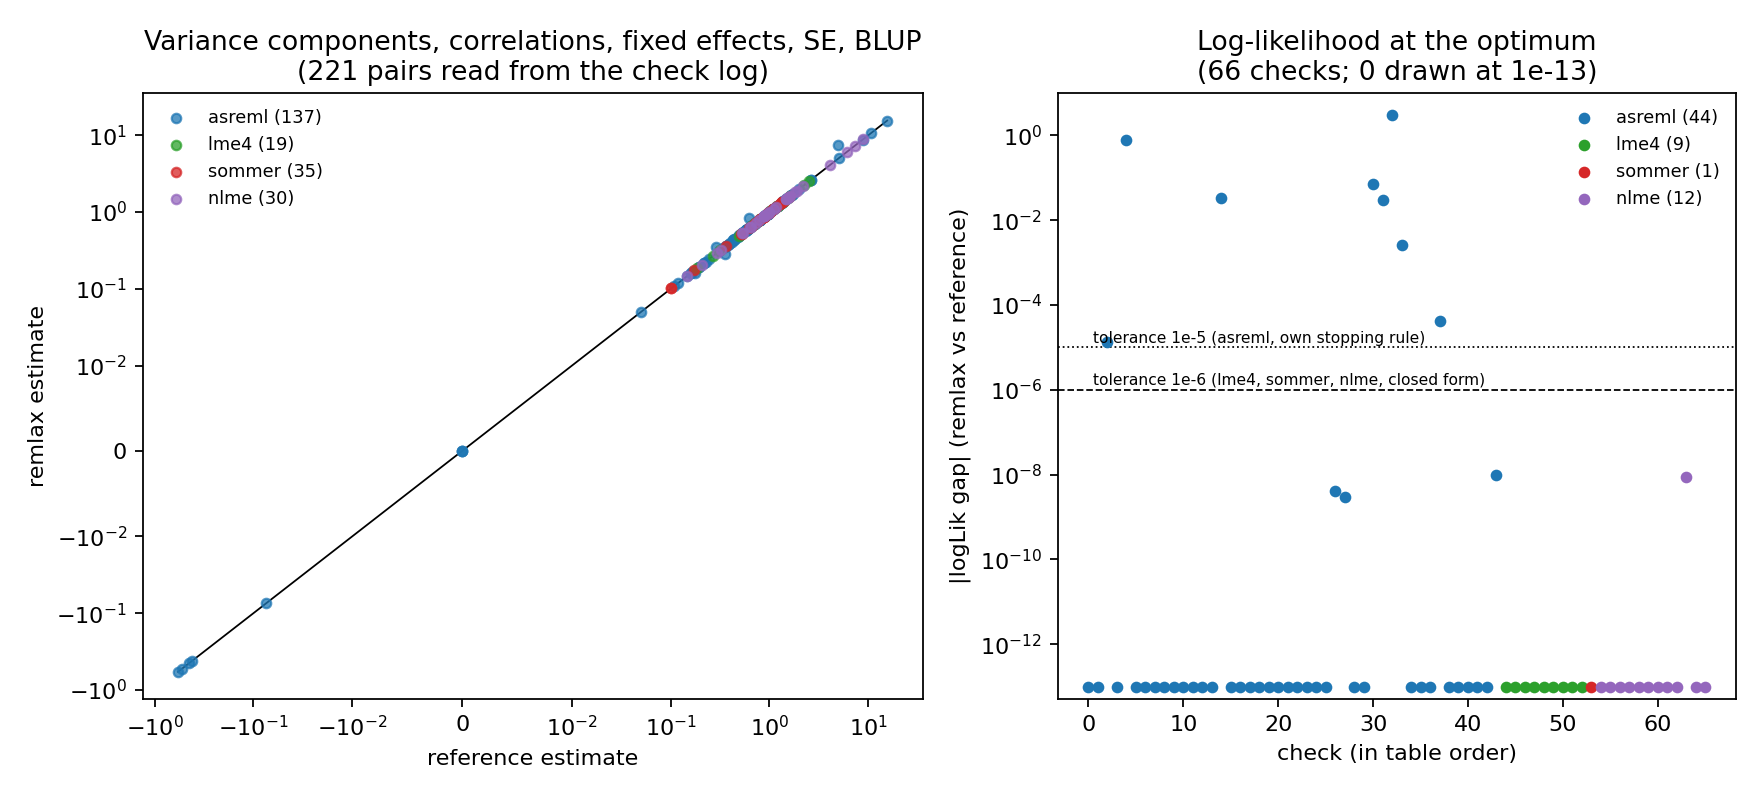
\includegraphics[width=\textwidth]{figures/fig_validation.png}
\caption{\label{fig:validation}Estimates of \pkg{remlax} against the
reference programs. Left, the 221 pairs of variance components,
correlations, fixed effects, standard errors and BLUPs printed by the checks.
Right, the absolute gap of log-likelihood at the optimum for the 66 checks
that print both values, with zeros drawn at $10^{-13}$. The points above
$10^{-5}$ are \code{ma2}, \code{sph} and \code{cir} against \pkg{asreml} and
\code{lvr} against a profile computed in \proglang{R}, and the point at
$4.3 \times 10^{-5}$ is \code{rr(1)}.}
\end{figure}

Twelve of the 17 failures came from the \pkg{asreml} suite, on the moving-average
residual \code{ma2} and on the spherical and circular kernels fitted to an
irregular field of 90 positions. Each model was handed to an independent
REML written in dense \proglang{R} algebra, and \pkg{asreml} was held at the
parameters of \pkg{remlax}. On \code{sph}, \pkg{asreml} reported
non-convergence and oscillated between two iterates. Held at the parameters
of \pkg{remlax}, it returned the log-likelihood of \pkg{remlax} to the last
digit. On \code{cir}, the likelihood has three local maxima in the range, at
5.0, 7.4 and 10.9. \pkg{asreml} stopped in the first and \pkg{remlax} reached
the highest, 3.03 units above. On \code{ma2}, \pkg{asreml} declared
convergence while its parameters still moved by 3.5\,\% per iteration, 0.033
units below \pkg{remlax}. In each case, the independent REML reproduced the
value of \pkg{remlax}. The rows are left as failures, since the criterion is
agreement with what \pkg{asreml} reports.

Five failures remain. On the two-dimensional P-spline, \pkg{asreml} received
the five basis matrices of the PS-ANOVA and stopped $1.4 \times 10^{-5}$
below \pkg{remlax}, with one variance 0.5\,\% apart. It stayed at that point
when allowed to iterate further. The truncated tent \code{lvr} has a
likelihood with one local maximum per integer range. \pkg{remlax} stopped at
a range of 1.51, 0.76 units below the maximum found by a fine grid in
\proglang{R}, and \pkg{asreml} stopped lower still. On the anisotropic
Mat\'ern, the CPU/GPU check could not run, because the gradient is not finite
at zero distance and the fit is refused at its start. Finally, one of the 600
configurations of the random sweep ended with a Newton decrement of 0.011,
above the threshold of 0.01.

On the full direct and indirect genetic effects model of \citet{salas2026},
simulated on 600 plots, both programs placed the direct and indirect genetic
correlation at the boundary, $-1$. \pkg{remlax} reached a log-likelihood
higher by 0.02. The eight components agreed within 0.1 standard error, and
one indirect variance differed by 8\,\% (0.163 against 0.176, with a standard
error of 0.35).

This validation also revealed defects in \pkg{remlax}, all fixed since.
Metric structures written as $\rho^d$ started at $\rho = 0$, a point where
the gradient is zero by construction, so that L-BFGS-B stopped at once. In
addition, the gradient of the circular kernel was not finite beyond the range.
Range kernels also proved multimodal, which led to the sweep of starting
values of Section~\ref{sec:optim}.

\subsection{Internal agreement and simulation}

The mixed model engine and the AI optimiser were also checked directly. Their agreement with the dense engine was checked directly. The mixed model
engine returns the likelihood, gradient and AI matrix of the dense engine to
$10^{-13}$, and its prediction error variances to $3 \times 10^{-15}$. On
33 of 34 serialised designs fitted on both devices, the CPU and GPU values of
$-2\ell_R$ differed by at most $6.8 \times 10^{-16}$ in relative value, on
30 October 2026. A later check on an NVIDIA L40S, on 27 October 2026, found
seven benchmark designs in agreement to $10^{-13}$ at a common $\theta$, and
complete fits to $2 \times 10^{-10}$.

Our simulation suite covers 37 model types. They range from one random factor
to multi-trait \code{fa} models, separable residual fields, pedigrees given by
their precision, metric kernels and direct and indirect genetic effects in a
mixture of two species. Each data set was simulated from known parameters and
fitted by L-BFGS-B and by AI on the dense engine, and by AI on the mixed model
engine with automatic and with sparse inversion. An
independent dense REML written in \proglang{R} recomputed the log-likelihood at each estimate. A
fit passed when this arbiter agreed with the reported log-likelihood to
$10^{-8}$ in relative value, when the routes agreed to $10^{-4}$, when the
convergence criteria held, and when every component lay within three standard
errors of its true value. On 27 October 2026, 145 of 150 fits passed. All
four failures came from one factor analytic model, fitted along every route,
where one component lay at 3.06 standard errors with the same exact
likelihood. The last fit was an expected refusal, since AI is not used with a
spatial lag. Across all fits, the largest gap to the arbiter was $1.3 \times
10^{-11}$ in relative value, and the routes agreed within $6.5 \times
10^{-7}$. Beyond these checks, the package carries about 870 \pkg{testthat}
expectations and about 265 \pkg{pytest} tests.

%% =========================================================================
\section{Benchmarks}\label{sec:benchmarks}

\subsection{Design and hardware}

The benchmark compared \pkg{remlax} with \pkg{kmmr} \citep{melsen2026} and
\pkg{ASReml-R} on 30 simulated genomic problems. Each problem follows
\begin{equation}\label{eq:simmodel}
  y = \mu_{\rm env} + g + e, \qquad g \sim \mathcal{N}(0, \Sigma_g \otimes K),
  \qquad e \sim \mathcal{N}(0, \sigma^2_{\rm env}) \text{ within each
  environment}.
\end{equation}
The relationship matrix $K$ was a \citet{vanraden2008} matrix from 3000
markers drawn in 10 subpopulations, with $K = 0.98\,G/\overline{\diag G} +
0.02\,I$. The genetic covariance $\Sigma_g$ was built from two loadings per
environment plus a small diagonal, with unit variances, so that it is close to
rank two. Some problems vary the number of observations for a single trait,
with $q = 2000$ genotypes fixed or with $q = n/4$. Others vary the number of
variance parameters, with \code{us(t)} for $t = 1$ to 12 environments, or with
\code{diag}, \code{fa1}, \code{fa2}, \code{fa3} and \code{us} on the same data
with $t = 8$. Large values of $\dimC(C)/n$ arise when 1000 genotypes are
phenotyped among 1000 to 16\,000 in the relationship matrix, and in sparse
\code{fa2} trials over 10 environments that observe 100\,\% to 10\,\% of
the (genotype, environment) pairs.

Each point had three simulated data sets. Reported times are the median over
the data sets and replicates, and log-likelihoods were compared on the first
data set. The time of \pkg{remlax} is the whole \code{rx_fit()} call, start of
the \proglang{Python} server included, with a filled compilation cache. For
\pkg{kmmr} and \pkg{ASReml-R}, the times include the inversion of $K$ and the
starting values computed in \proglang{R}. \pkg{remlax} ran along an MME route,
with the mixed model engine, automatic inversion and AI, and along a V route,
with the dense engine in standard memory mode and AI. Neither route computed
the final Hessian or the BLUPs. \pkg{kmmr} ran
with a tolerance of $10^{-6}$ on the log-likelihood and at most 50 iterations,
and \pkg{ASReml-R} with at most 50 iterations and a 30\,GB workspace. Each fit
was limited to 6\,h.

\pkg{remlax} and \pkg{kmmr} ran on the genotoul cluster, on 8 cores of an AMD
EPYC 7513 node with 96\,GB of memory, or on one NVIDIA A100 80\,GB with 8 cores.
\pkg{ASReml-R} ran on the meso cluster, where its licence is available, on a
reserved node with the three programs pinned to the same 8 cores of one socket.
That node ran \pkg{remlax} 1.3 to 3 times faster than genotoul, so the
comparison with \pkg{ASReml-R} is biased against \pkg{remlax}. All runs used
the same container image.
%% TODO: CPU model of the A100 node (gpu01) and of the reserved meso node;
%% versions of kmmr (commit), ASReml-R, JAX and CUDA in the benchmark image;
%% remlax revision of the v14 runs.
At the time of writing, \pkg{ASReml-R} had completed 21 of the 30 problems,
since its licence forced the runs in series.
%% TODO: update when the remaining ASReml-R runs on meso have finished.

\subsection{Time against the number of observations}

Figure~\ref{fig:n} shows the time against $n$ for a single trait. With $q =
2000$ fixed, $\dimC(C)$ stays at 2001 and the MME route was flat. It took 4.0
to 9.8\,s on CPU from $n = 2000$ to $128\,000$, and 7.7 to 7.9\,s on the A100.
\pkg{kmmr} took 4.1 to 6.7\,s on CPU. The V route grew with $n$, from 9.6\,s at
$n = 2000$ to 3800\,s at $n = 32\,000$ on CPU, and from 13.8 to 216\,s on the
A100. One evaluation of the V form took 0.60\,s on CPU and 0.011\,s on the
A100 at $n = 2000$, and 558\,s and 6.9\,s at $n = 32\,000$. At $n \ge 64\,000$, the V form ran out of the 96\,GB of
memory on CPU. These runs were not attempted on the A100, since three matrices
of order 64\,000 exceed its 80\,GB. With $q = n/4$, it also ran out of memory on
the A100 at $n = 32\,000$. \pkg{ASReml-R} took 12.3 to 13.4\,s
up to $n = 8000$.

With $q = n/4$, $\dimC(C)$ grows with $n$. At $n = 64\,000$ and $q =
16\,000$, the MME route took 223\,s on CPU and 63.9\,s on the A100, against
571\,s and 245\,s for \pkg{kmmr}. On small problems, \pkg{remlax} pays a fixed
cost. Every fit on the A100 took at least 7.2\,s, where \pkg{kmmr} took 2.3\,s
at $n = 2000$.

\begin{figure}[p]
\centering
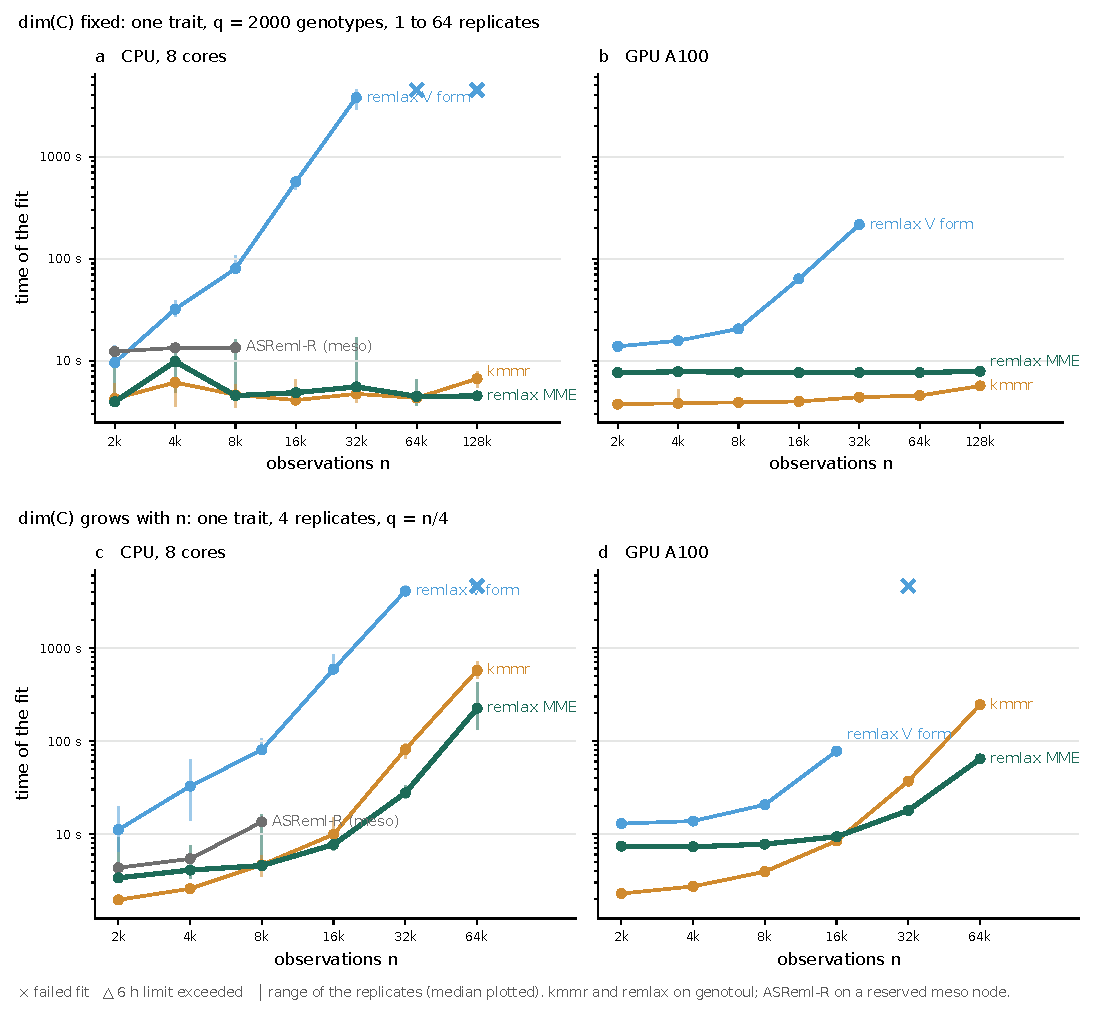
\includegraphics[width=\textwidth]{figures/fig_temps_n.pdf}
\caption{\label{fig:n}Time of the fit against the number of observations,
single-trait genomic BLUP. Top, $q = 2000$ genotypes and 1 to 64 replicates.
Bottom, 4 replicates and $q = n/4$. Left, 8 CPU cores; right, one A100. Each
point is the median of the replicates, and vertical bars give their range.
Crosses mark failed fits. \pkg{ASReml-R} ran on another cluster, faster than
the one used for \pkg{remlax} and \pkg{kmmr}.}
\end{figure}

\subsection{Time against the number of variance parameters}

Figure~\ref{fig:p} shows the time against the number $p$ of variance
parameters. With \code{us(t)}, $n$ and $\dimC(C)$ grow with $t$. At $t = 8$
($p = 44$), the MME route took 64.8\,s on the A100 and 1887\,s on CPU.
\pkg{ASReml-R} took 3187\,s and stopped 3.79 log-likelihood units below the
best value, and \pkg{kmmr} failed. At $t = 12$ ($p = 90$), the MME and V routes
took 143 and 140\,s on the A100, and \pkg{kmmr} failed again. On the same data
with $t = 8$, the MME route on the A100 took 9.3\,s for \code{fa1}, 10.8\,s for
\code{fa2} and 12.6\,s for \code{fa3}. \pkg{ASReml-R} took 61.2, 161 and
582\,s for the same structures, and \pkg{kmmr} on the A100 took 34.5, 70.8 and
155\,s. On \code{fa2}, \pkg{kmmr} stopped 0.31 units below the best value. With 8
CPU cores, the MME route was close to \pkg{kmmr} for the factor analytic models,
with 42.7 to 145\,s against 50.4 to 179\,s.

\begin{figure}[p]
\centering
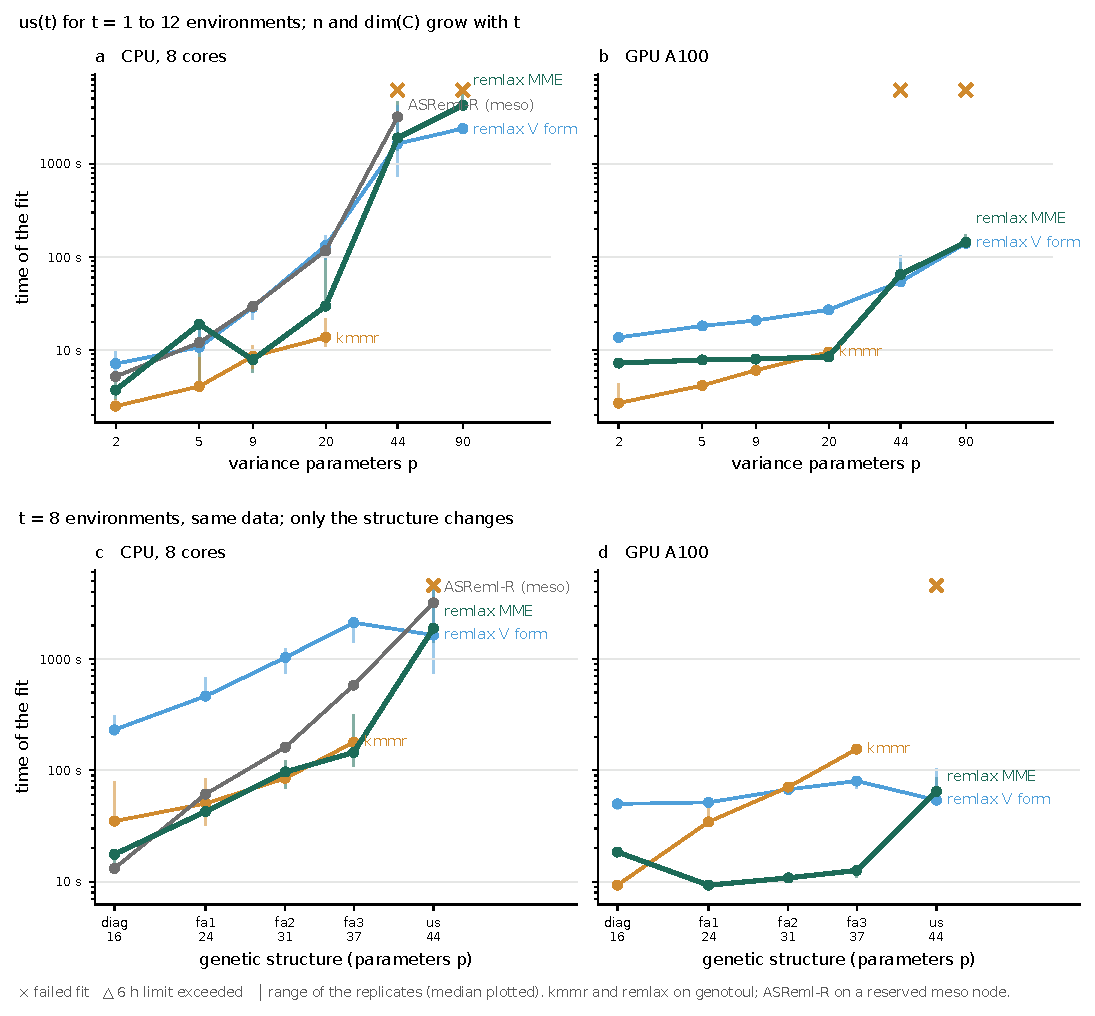
\includegraphics[width=\textwidth]{figures/fig_temps_p.pdf}
\caption{\label{fig:p}Time of the fit against the number of variance
parameters $p$. Top, \code{us(t)} for $t = 1$ to 12 environments with $q =
1000$ and one observation per (genotype, environment) pair, so that $n$ and
$\dimC(C)$ grow with $t$. Bottom, $t = 8$ on the same data, only the genetic
structure changing. Layout as in Figure~\ref{fig:n}.}
\end{figure}

\subsection{When C becomes large against n}

Figure~\ref{fig:C} covers the regime where $\dimC(C)$ is large against $n$.
With 1000 phenotyped genotypes among 16\,000 in the relationship matrix,
$\dimC(C)/n = 16$. \pkg{ASReml-R} then took 4026\,s, \pkg{kmmr} 552\,s on CPU
and 232\,s on the A100, and the MME route 128\,s and 63.2\,s. The V route
factorises a matrix of order $n = 1000$ only, and took 14.6\,s on CPU and
21.1\,s on the A100. In the sparse trials with 10\,\% of the pairs observed
($n = 2000$, $\dimC(C) = 20\,010$), the V route took 31.1\,s on the A100 and
519\,s on CPU, against 311\,s and 6724\,s for the MME route. \pkg{ASReml-R}
took 5013\,s and \pkg{kmmr} failed. With all pairs observed ($n = 20\,000$),
the MME route took 34.8\,s on the A100, against 407\,s for \pkg{kmmr}.

Figure~\ref{fig:rule} compares the cost of one evaluation of the two forms on
every problem. On CPU, the dense MME evaluation was cheaper than the V
evaluation on every problem with $\dimC(C)/n \le 2$ except \code{us(12)},
where it cost 2\,\% more. Above $\dimC(C)/n = 4$, the V evaluation
was cheaper on every problem but one, the sparse trial with 10\,\% of the
pairs observed. The automatic choice of engine does not yet read
$\dimC(C)/n$, and takes the MME route whenever the model is in its scope.

\begin{figure}[p]
\centering
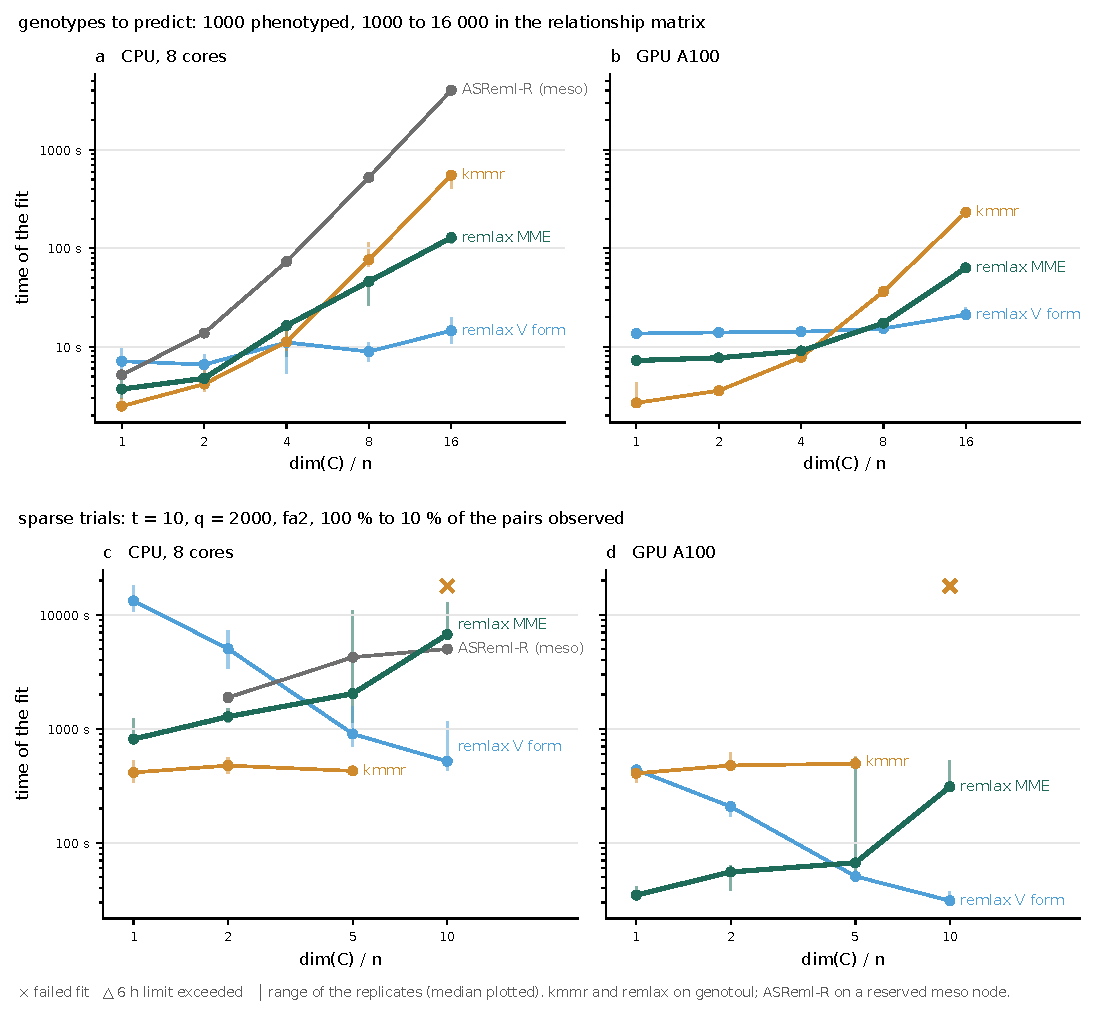
\includegraphics[width=\textwidth]{figures/fig_temps_C.pdf}
\caption{\label{fig:C}Time of the fit when $\dimC(C)$ becomes large against
$n$. Top, 1000 phenotyped genotypes among 1000 to 16\,000 in the relationship
matrix. Bottom, sparse \code{fa2} trials over 10 environments and 2000
genotypes, from 100\,\% to 10\,\% of the pairs observed. Layout as in
Figure~\ref{fig:n}.}
\end{figure}

\begin{figure}[t]
\centering
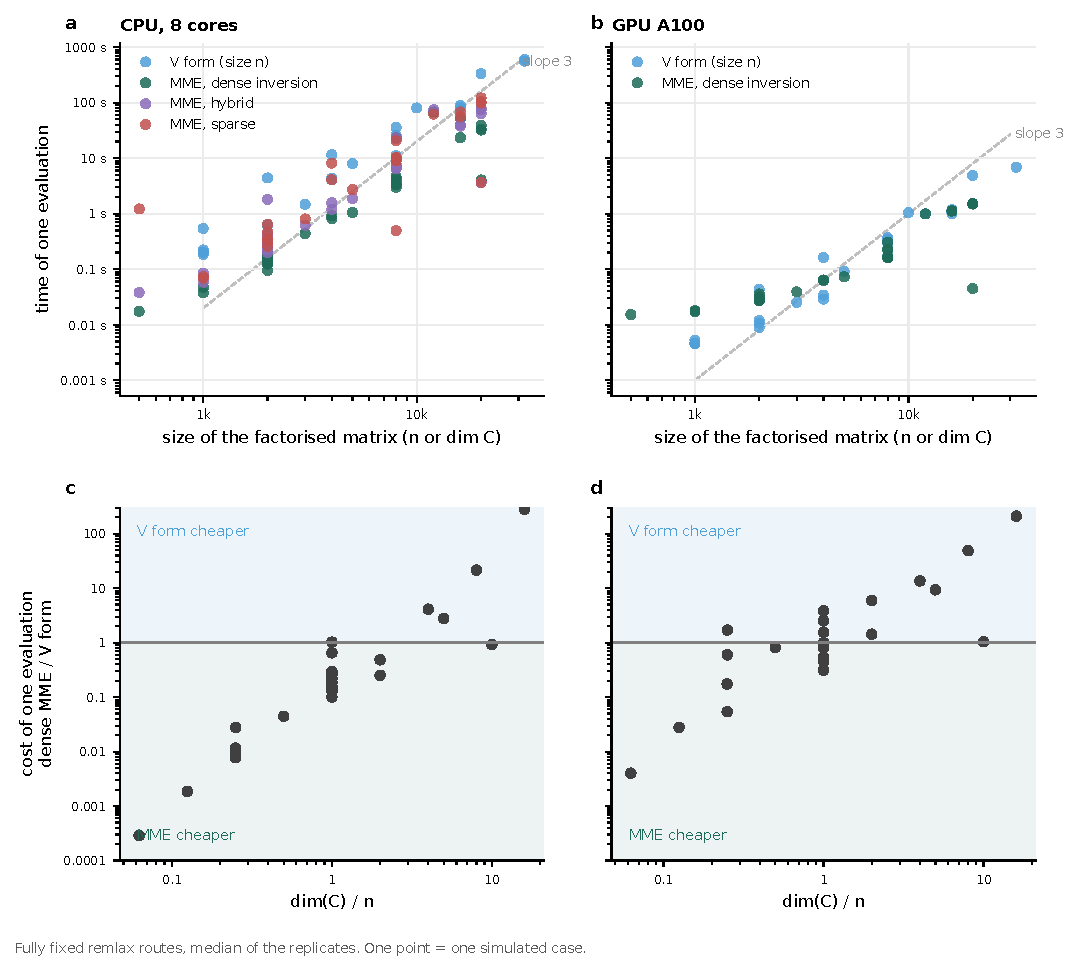
\includegraphics[width=\textwidth]{figures/fig_regle.pdf}
\caption{\label{fig:rule}Cost of one evaluation in the \pkg{remlax} routes
with every option fixed. Top, time of one evaluation against the order of the
factorised matrix, $n$ for the V form and $\dimC(C)$ for the MME form, with a
reference line of slope 3. Bottom, ratio of the cost of a dense MME
evaluation to that of a V evaluation against $\dimC(C)/n$. Left, 8 CPU cores;
right, one A100. One point per simulated problem, median of the replicates.}
\end{figure}

\subsection{CPU against GPU}

Figure~\ref{fig:gpu} gives the speed-up of the A100 over 8 CPU cores for each
route. With a single trait and at most 2000 genotypes, the MME route was faster on
CPU in all problems but one, with speed-ups of 0.46 to 0.72. The fixed cost of
the GPU dominates these fits. Speed-ups grew with the size of the dense blocks of $C$. They reached
3.5 at $q = 16\,000$, 4.6 to 11.5 for the factor analytic models with $t = 8$,
and 21.7 to 30.4 for \code{us(8)}, \code{us(12)} and the sparse trials. The V
route gained 17.6 at $n = 16\,000$ for a single trait, and 30.3 on
\code{us(8)}. \pkg{kmmr} gained 0.85 to 3.8 from its GPU on these problems.

\begin{figure}[t]
\centering
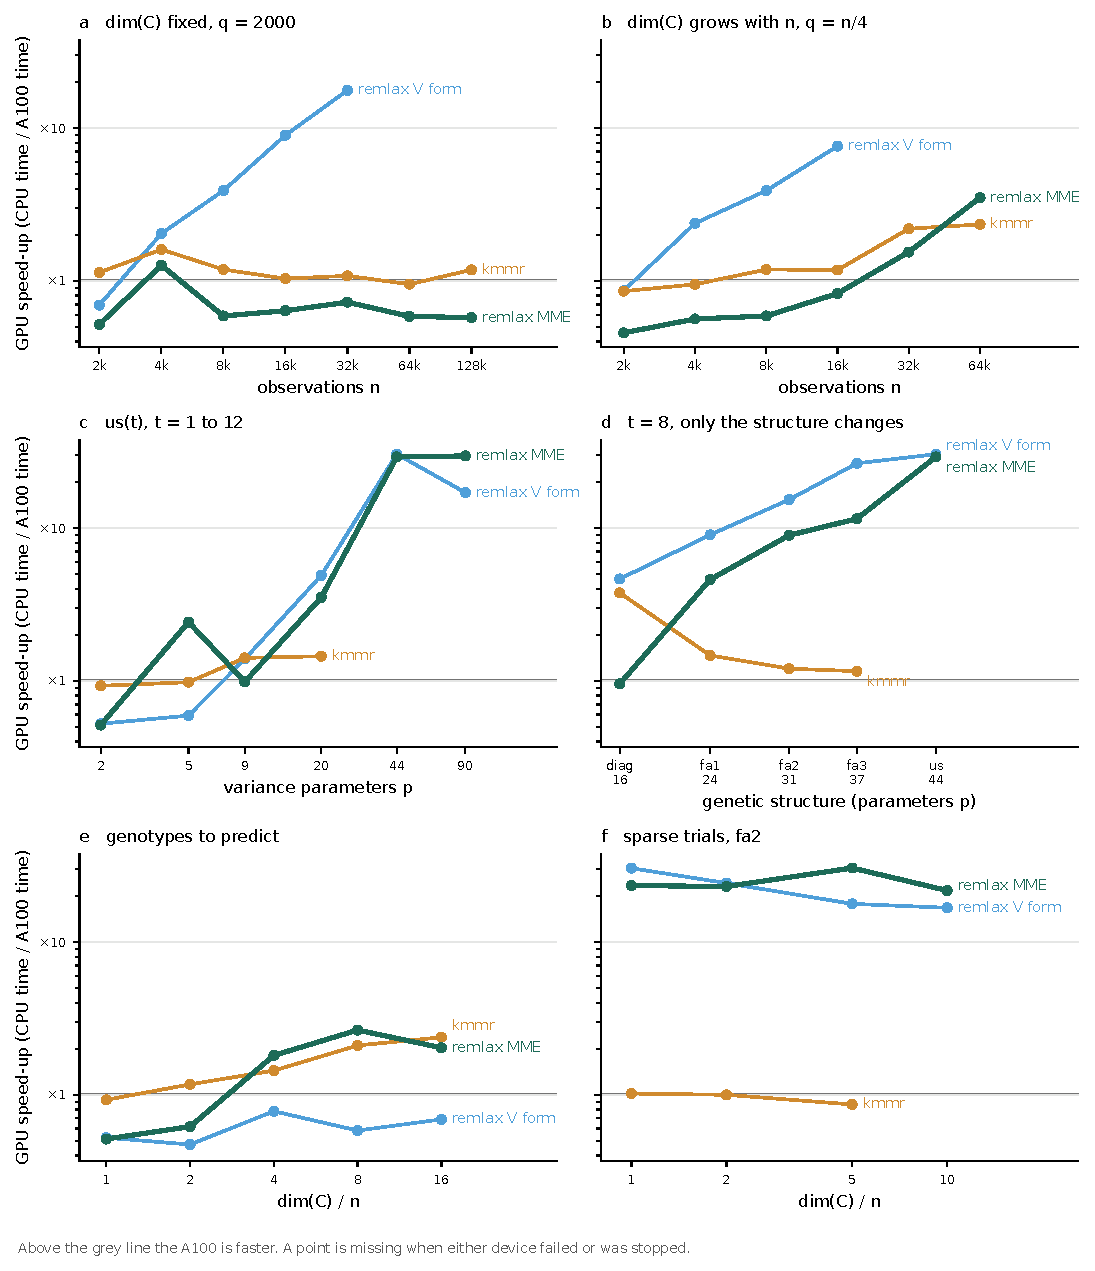
\includegraphics[width=\textwidth]{figures/fig_cpu_gpu.pdf}
\caption{\label{fig:gpu}Speed-up of one A100 over 8 CPU cores, CPU time
divided by A100 time, for the same route and problem. Above the grey line, the
A100 is faster. A point is missing when either device failed.}
\end{figure}

\subsection{remlax against ASReml-R}

Figure~\ref{fig:asreml} pairs each of the 21 problems completed by
\pkg{ASReml-R} with the MME route of \pkg{remlax}. On the A100, \pkg{remlax}
was faster on 17 of them, by factors up to 49 on \code{us(8)} and 64 at
$\dimC(C)/n = 16$. It was slower on three single-trait problems that
\pkg{ASReml-R} fitted in 4.3 to 5.4\,s, below the fixed cost of about 7\,s of
\pkg{remlax}, and on the \code{diag} model with $t = 8$. On CPU,
\pkg{remlax} was faster on 18 of the 21 problems, despite the slower node.

\begin{figure}[t]
\centering
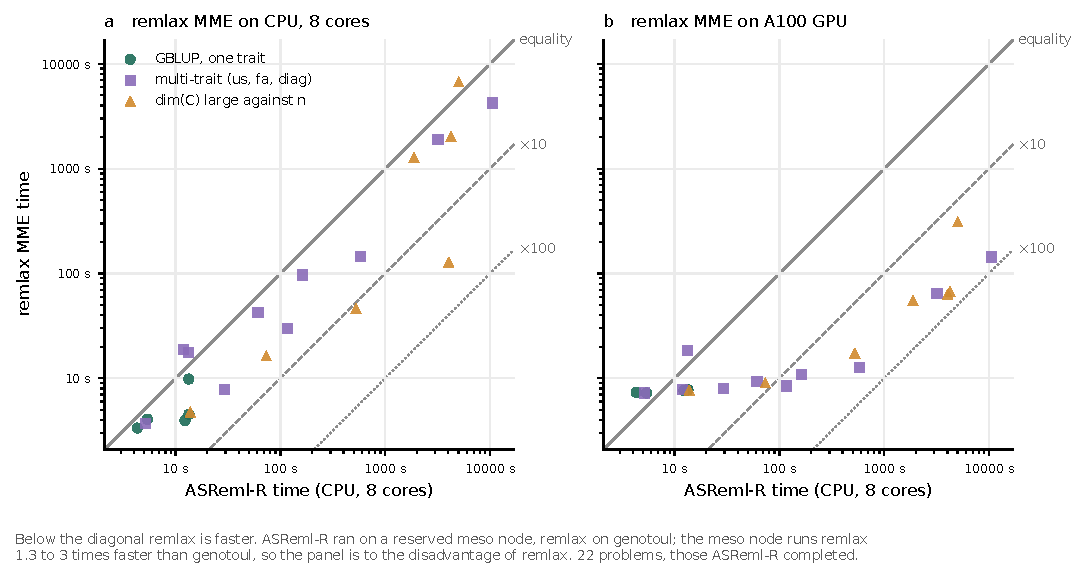
\includegraphics[width=\textwidth]{figures/fig_remlax_asreml.pdf}
\caption{\label{fig:asreml}Time of the MME route of \pkg{remlax} against
\pkg{ASReml-R} on the same problems. Left, \pkg{remlax} on 8 CPU cores; right,
on one A100. \pkg{ASReml-R} ran on 8 cores of a reserved node that ran
\pkg{remlax} 1.3 to 3 times faster than the node used for \pkg{remlax}. Below
the diagonal, \pkg{remlax} is faster.}
\end{figure}

\subsection{Real data}

Table~\ref{tab:real} reports fits to real data with a development version of
\pkg{remlax} frozen on 27 October 2026.
%% TODO: rerun these seven models with the released version.
The DROPS data hold maize hybrids in European trials
\citep{millet2016,millet2019}, analysed in two stages or in one stage with
AR(1) $\times$ AR(1) fields per trial. In the wheat data, lines were grown
under five treatments \citep{krause2019}. On every model, \pkg{remlax} reached an optimum
at least as high as those of \pkg{kmmr} and \pkg{ASReml-R}, and strictly
higher on four of them. With the A100, it fitted the \code{fa2} model over five treatments in
44.4\,s against 961\,s for \pkg{kmmr}, 20 units higher. On 8 CPU cores,
\pkg{remlax} was slower than \pkg{kmmr} on that model, 995\,s against 813\,s.
\pkg{ASReml-R} capped the AR(1) correlations of the one-stage DROPS models at
0.98. With these correlations fixed at 0.98 in \pkg{remlax} as well, the two
optima agreed to within 0.02.

\begin{table}[t]
\centering
\footnotesize
\setlength{\tabcolsep}{4pt}
\begin{tabular}{lrrrrrrrr}
\toprule
 & \multicolumn{3}{c}{Log-likelihood} & \multicolumn{3}{c}{CPU, 8 cores (s)} & \multicolumn{2}{c}{A100 (s)} \\
\cmidrule(lr){2-4}\cmidrule(lr){5-7}\cmidrule(lr){8-9}
Model & \pkg{kmmr} & \pkg{ASReml-R} & \pkg{remlax} & \pkg{kmmr} & \pkg{remlax} & \pkg{ASReml-R} & \pkg{kmmr} & \pkg{remlax} \\
\midrule
DROPS 2-stage, \code{fa1} & $-492.86$  & $-492.86$  & $-492.86$  & 6.2 & 7.2 & 0.5 & 8.3 & 8.2 \\
DROPS 2-stage, \code{fa3} & $-368.06$  & $-378.25$  & $-367.68$  & 16.0 & 9.7 & 2.4 & 19.6 & 10.0 \\
DROPS 1-stage, \code{fa1} & $-2154.65$ & $-1161.86$ & $-1161.21$ & 3.9 & 29.1 & 15.3 & 5.0 & 42.7 \\
DROPS 1-stage, \code{us(5)} & $-2169.30$ & $-1146.72$ & $-1146.19$ & 5.8 & 18.0 & 10.5 & 5.6 & 28.3 \\
Wheat, GBLUP                 & 389.57 & 389.57 & 389.57 & 9.1 & 9.0 & 60.2 & 7.4 & 9.2 \\
Wheat, \code{fa2} & 7109.92 & 7126.36 & 7130.18 & 813 & 995 & 7429 & 961 & 44.4 \\
Wheat, \code{us(5)} & 7138.93 & 7138.93 & 7138.93 & 359 & 316 & 7530 & 82.6 & 22.1 \\
\bottomrule
\end{tabular}
\caption{\label{tab:real}Seven models on real data. Both \pkg{kmmr} and
\pkg{remlax} ran on the same genotoul nodes, and \pkg{ASReml-R} on meso,
where its times are orders of magnitude only. \pkg{kmmr} stopped after two
iterations on the one-stage DROPS models. Log-likelihoods are in the
convention of \pkg{ASReml-R}. The wheat models cover five treatments.}
\end{table}

%% =========================================================================
\section{Limitations and availability}\label{sec:limits}

\subsection{Experimental features}

Several features have been used on few data sets, and their interface may
change without a deprecation period. This group includes the hybrid
inversion and the blocks engine (Section~\ref{sec:computation}). Only
L-BFGS-B drives the blocks engine, which has not yet been compared with the
mixed model engine.

The Bayesian route samples the posterior of the variance parameters by
Hamiltonian Monte Carlo, with the fixed and random effects integrated out
analytically. Many short chains share one trajectory length, adapted by the
ChEES criterion \citep{hoffman2021}, and advance together in vectorised calls
of \pkg{BlackJAX} \citep{cabezas2024} on CPU or GPU. The chains work on
whitened parameters, with the Laplace covariance at the posterior mode or at
the REML optimum. Convergence is judged by the nested $\hat R$ of
superchains \citep{margossian2024}. Half-$t$, half-normal, half-Cauchy,
inverse gamma or flat priors apply to standard deviations, LKJ priors to the
correlations of \code{us} blocks, and normal priors to loadings. On a model with
400 observations, 8 chains of 100 draws took 50\,s on a laptop CPU, with an
effective sample size above 550 for every component. Its posterior is always
evaluated by the dense engine.

The spatial lag of the response fits the structural model $y = My + X\beta +
Zu + e$, with $M_{(t,i),(u,j)} = \Psi_{tu} W_t[i,j]$ and $\Psi$ estimated with
the variance parameters. By default, the criterion is the exact restricted
likelihood of $y$, including $\log|\det(I - M)|$ and the term of
\citet{harville1977} that depends on $\Psi$. This structural model runs on
the dense engine only. Against an independent engine, on three data sets, two criteria and
three models, log-likelihoods agreed within $8 \times 10^{-7}$.

Genome-wide scans test every marker at the variance components of a fitted
model, for direct effects, indirect effects and their joint test. The scan
with one null model per chromosome and the exact refit of the top markers with
re-estimated components are experimental. At fixed $V$, the $p$-value of a
marker with a large effect was about 6 times too large, which the refit
removes.

\subsection{Limitations}

The dense engine forms $V$, so its memory grows as $n^2$ and its time as
$n^3$. For a single trait, the V route ran out of memory at $n = 32\,000$ on
the A100 80\,GB when $q = 8000$, and at $n = 64\,000$ with 96\,GB of CPU
memory. Large $n$ with a small or sparse $C$ belongs to the mixed model engine.
The automatic choice of engine ignores $\dimC(C)/n$, although the V form was
cheaper when $C$ was much larger than $n$ (Figure~\ref{fig:rule}). A fixed
cost of about 7\,s per fit on GPU, for compilation and transfers, makes it
slower than 8 CPU cores on small models. The Kenward--Roger adjustment omits
the second-order term. Wald tests are conditional, whereas the default of
\pkg{ASReml-R} is sequential, and the two agree on the last term of the model.
Generalised linear mixed models are not covered. The \code{ilv} structure of
\pkg{ASReml-R} is absent, since its formula could not be recovered. Ranges of
neighbour kernels are profiled over a grid and not estimated by REML.

Reproducibility has limits set by floating point arithmetic. CPU fits are
bitwise reproducible on one core and reproducible to about $10^{-13}$ in
relative value on several cores. On GPU, reductions are not deterministic.
Two identical fits on an RTX A1000 agreed on $-2\ell_R$ to $3 \times 10^{-13}$
but stopped at points $2 \times 10^{-8}$ apart on the same flat top. An
evaluation at a fixed $\theta$ is exact on both devices.

\subsection{Availability}

\pkg{remlax} is distributed under the GNU General Public License, version 3 or
later, at \url{https://github.com/NicoSalas34/remlax}. It installs with
\begin{Code}
remotes::install_github("NicoSalas34/remlax", build_vignettes = TRUE)
\end{Code}
It needs \proglang{Python} 3.10 or later with \pkg{jax} 0.4.30, \pkg{numpy}
1.24 and \pkg{scipy} 1.10 or later. On request, \code{rx_install_python()}
creates such an environment, with the CUDA build of \pkg{JAX} for GPU fitting.
Optional modules add the nested dissection order and \pkg{CHOLMOD}
(\pkg{pymetis}, \pkg{cvxopt}) and the Bayesian route (\pkg{blackjax}). The
vignettes document the formula grammar, the structure catalogue, every
function of the engine and the validation. Scripts of the validation and of
the benchmarks are in the repository
\url{https://github.com/NicoSalas34/remlax-validation}.

\section*{Acknowledgements}
%% TODO: acknowledgements, funding and computing resources (genotoul
%% bioinformatics platform, meso@LR).

\bibliography{remlax}

\end{document}
